\chapter{Specifikacija programske potpore}
		
	\section{Funkcionalni zahtjevi}
	
			\noindent \textbf{Dionici:}
			
			\begin{packed_enum}
				
				\item Administrator-voditelj tima
				\item Razvojni tim CodeCooks			
				\item Profesori predmeta Programsko inžinjerstvo
				\item Korisnici
				
			\end{packed_enum}
			
			\noindent \textbf{Aktori i njihovi funkcionalni zahtjevi:}
			
			
			\begin{packed_enum}
				\item  \underbar{Admin može:}
				
				\begin{packed_enum}
					
					\item Upravljanje korisnicima
					\item Upravljanje receptima
					\begin{packed_enum}
						
						\item  Brisanje recepata
						\item  Uređivanje recepata
						
					\end{packed_enum}
					\item Upravljanje komentarima
					\begin{packed_enum}
						
						\item  Brisanje komentara 
						\item  Cenzuriranje komentara
				
					\end{packed_enum}
					\item  Mjenjanje kategorija
					
				\end{packed_enum}
			
				\item  \underbar{Registrirani korisnik može:}
				
				\begin{packed_enum}
					
					\item Objavljivanje recepata
					\item Komuniciranje s ostalim registriranim korisnicima
					\item Objavljivanje termina za komunikaciju
					\item Označavanje recepata
					\item Komentiranje recepata
					\item Spremanje recepata
					\item Praćenje drugih registriranih korisnika
					\item Upravljanje dozvolama pratiteljima
					\item Upravljanje osobnim informacijama
					\item Upravljanje postavkama komunikacije i obavijestima
					
				\end{packed_enum}
				
				\item  \underbar{Neregistrirani korisnik može:}
				
				\begin{packed_enum}
					
					\item Pregledavanje recepata temeljem kategorija
					
				\end{packed_enum}
				
				
				\item  \underbar{Baza podataka može:}
				
				\begin{packed_enum}
					
					\item Pohrana osobnih podataka registriranog korisnika
					\item Pohrana recepata
					\item Pohrana komentara
					
				\end{packed_enum}
			\end{packed_enum}
			
			\eject 
			
			
				
			\subsection{Obrasci uporabe}
				
				
						\noindent \underbar{\textbf{UC1 - Pregled recepata}}
					\begin{packed_item}
						
						\item \textbf{Glavni sudionik: Neregistiran korisnik, Registriran korisnik}
						\item  \textbf{Cilj: Pregled recepata temeljem kategorija} 
						\item  \textbf{Sudionici: Baza podataka} 
						\item  \textbf{Preduvjet: -} 
						\item  \textbf{Opis osnovnog tijeka:}
						
						\item[] \begin{packed_enum}
							
							\item Korisnik otvori platformu.
							\item Ponuđene su mu kategorije, vrste kuhinje, specifični sastojci.
							\item Korisnik odabire kategoriju.
							\item Prikazuju mu se recepti.
							\item Korisnik odabire recept.
							\item Recept se prikazuje u web sučelju.
						\end{packed_enum}
						
						\item  \textbf{Opis mogućih odstupanja:}
						
						\item[] \begin{packed_item}
							
							\item[3.a] Nema pohranjenih recepata vezanih za zadanu kategoriju te se korisnik obavještava da nema podataka za njegovu pretragu.
							
							
						\end{packed_item}
					\end{packed_item}
					
					
					\noindent \underbar{\textbf{UC2 - Registracija}}
					\begin{packed_item}
						
						\item \textbf{Glavni sudionik: Neregistrirani korisnik}
						\item  \textbf{Cilj: Stvaranje računa za pristup ostalim značajkama sustava}  
						\item  \textbf{Sudionici: Baza podtaka} 
						\item  \textbf{Preduvjet:-} 
						\item  \textbf{Opis osnovnog tijeka:}
						
						\item[] \begin{packed_enum}
							
							\item Korisnik odabire opciju za registraciju
							\item Korisnik unosi potrebne korisničke podatke
							\item Korisnik prima obavijest o uspješnoj registraciji
						\end{packed_enum}
						
						\item  \textbf{Opis mogućih odstupanja:}
						
						\item[] \begin{packed_item}
							
							\item[2.a] Odabir već zauzetog korisničkog imena i/ili e-maila, unos korisničkog podatka u nedozvoljenom formatu ili pružanje neispravnoga e-maila.
							\item[] \begin{packed_enum}
								
								\item  Sustav obavještava korisnika o neuspjelom upisu i vraća ga na stranicu za registraciju.
								\item Korisnik mijenja potrebne podatke te završava unos ili odustaje od registracije.
								
							\end{packed_enum}
							
						\end{packed_item}
					\end{packed_item}
					
					
					\noindent \underbar{\textbf{UC3 - Prijava u sustav}}
					\begin{packed_item}
						
						\item \textbf{Glavni sudionik: Neregistrirani korisnik}
						\item  \textbf{Cilj: Prijava korisnika u sustav} 
						\item  \textbf{Sudionici: Baza podataka} 
						\item  \textbf{Preduvjet:} 
						\item  \textbf{Opis osnovnog tijeka:}
						
						\item[] \begin{packed_enum}
							
							\item Korisnik odabire opciju za prijavu.
							\item Korisnik unosi potrebne korisničke podatke.
							\item Korisnik dobiva potvrdnu poruku o prijavi.
							\item Otvara se početni zaslon za registriranog korisnika.
							
						\end{packed_enum}
						
						\item  \textbf{Opis mogućih odstupanja:}
						
						\item[] \begin{packed_item}
							
							\item[2.a] Upis pogrešnog korisničkog imena ili lozinke.
							\item[] \begin{packed_enum}
								
								\item  Sustav obavještava korisnika o neuspjeloj prijavi i vraća ga na stranicu za prijavu.
								
							\end{packed_enum} 
							
						\end{packed_item}
					\end{packed_item}
					
					\noindent \underbar{\textbf{UC4 - Objava recepata}}
					\begin{packed_item}
						
						\item \textbf{Glavni sudionik: Registrirani korisnik }
						\item  \textbf{Cilj: Objava svog recepta na stranici} 
						\item  \textbf{Sudionici: Baza podataka} 
						\item  \textbf{Preduvjet: Registracija i prijava korisnika} 
						\item  \textbf{Opis osnovnog tijeka:}
						
						\item[] \begin{packed_enum}
							
							\item Korisnik odabire opciju objava recepta.
							\item Aplikacija prikaže formu za objavu recepta.
							\item Korisnik unosi potrebne podatke.
							\item Nakon potvrde objave, otvara se početni zaslon za registriranog korisnika.
						\end{packed_enum}
						
						\item  \textbf{Opis mogućih odstupanja:}
						
						\item[] \begin{packed_item}
							
							\item[2.a] Aplikacija ne učita sva polja forme, gdje je potrebno ponovno zahtjevanje forme za objavu recepta. 
							\item[3.a] Nisu ispunjeni svi potrebni podatci o receptu što vraća korisnika da dopuni nedostajeće podatke.
							
						\end{packed_item}
					\end{packed_item}
					
					\noindent \underbar{\textbf{UC5 - Razmjena poruka}}
					\begin{packed_item}
						
						\item \textbf{Glavni sudionik: Registrirani korisnici}
						\item  \textbf{Cilj: Razmjena poruka između registriranih korisnika} 
						\item  \textbf{Sudionici: Baza podataka} 
						\item  \textbf{Preduvjet: } 
						\item  \textbf{Opis osnovnog tijeka:}
						
						\item[] \begin{packed_enum}
							
							\item Korisnik otvara profil drugog korisnika.
							\item Korisnik odabire opciju za chat.
							\item Korisnik odabire vrstu chata(text, video, poziv).
							\item Otvara se zaslon za komunikaciju sa drugim korisnikom.
						
						\end{packed_enum}
						
						\item  \textbf{Opis mogućih odstupanja:}
						
						\item[] \begin{packed_item}
							 
							\item[3.a] Ne otvara zaslon za komunikaciju zbog velikog broja zahtjeva za razmjenom poruka.
							
						\end{packed_item}
					\end{packed_item}
					
					\noindent \underbar{\textbf{UC6 - Čavrljanje }}
					\begin{packed_item}
						
						\item \textbf{Glavni sudionik: Registrirani korisnici}
						\item  \textbf{Cilj: Razmjena tekstualnih poruka između korisnika} 
						\item  \textbf{Sudionici: Baza podataka, API} 
						\item  \textbf{Preduvjet: )} 
						\item  \textbf{Opis osnovnog tijeka:}
						
						\item[] \begin{packed_enum}
							
							\item Otvara se prozor za upis teksta određenog korisnika.
							\item Korisnik upisuje poruku.
							\item Korisnik šalje poruku čime se osvježava prozor za upis i čitanje poruka.
							 
						\end{packed_enum}
						
						\item  \textbf{Opis mogućih odstupanja:}
						
						\item[] \begin{packed_item}
							
							\item[3.a] Poruka nije uspješno poslana što vraća korisniku opciju za ponovno slanje.
							
						\end{packed_item}
					\end{packed_item}
					
					\noindent \underbar{\textbf{UC7 - Videopoziv}}
					\begin{packed_item}
						
						\item \textbf{Glavni sudionik: Registrirani korisnici}
						\item  \textbf{Cilj: Uspostava videopoziva između korisnika.} 
						\item  \textbf{Sudionici: Baza podataka, API} 
						\item  \textbf{Preduvjet:} 
						\item  \textbf{Opis osnovnog tijeka:}
						
						\item[] \begin{packed_enum}
							
							\item Otvara se prozor sa ponuđenim opcijama prilikom videopoziva.
							\item Korisnik odabere opcije te pokrene videopoziv i čeka na odgovor.
							\item Uspostavom poziva otvara se prozor sa videopozivom.
							\item Nakon završetka videopoziva, otvara se prozor odabira komunikacijskog sredstva sa drugim korisnikom.
						\end{packed_enum}
						
						\item  \textbf{Opis mogućih odstupanja:}
						
						\item[] \begin{packed_item}
							
							\item[2.a] Drugi korisnik ne odgovara na poziv u određenom vremenu te se poziv prekine i pošalje prikladnja povratna poruka.
							\item[2.b] Drugi korisnik je zauzet te ne može odgovoriti na poziv čime se šalje prikladna povratna poruka. 
							\item[3.a] Prevelika latencija poziva te dodatno usporavanje mreže te gubitak informacije gdje se pokušava ugasiti video, a ako se ne popravi, poziv se prekida i šalje se prikladna povratna poruka.
							
						\end{packed_item}
					\end{packed_item}
					
					
				\subsubsection{Dijagrami obrazaca uporabe}
					
					\textit{Prikazati odnos aktora i obrazaca uporabe odgovarajućim UML dijagramom. Nije nužno nacrtati sve na jednom dijagramu. Modelirati po razinama apstrakcije i skupovima srodnih funkcionalnosti.}
				\eject		
				
			\subsection{Sekvencijski dijagrami}
				
				\noindent
				\textbf{Obrazac uporabe UC1-Pregled recepata}\newline
					{Korisnik šalje zahtjev za prikaz recepata po kategorijama, sastojcima i/ili kuhinjama kojim pripadaju. Poslužitelj dohvaća recepete koji zadovoljavaju uvjete i prikazuje ih korisniku. Korisnik sada može spremiti recepte, ako je prijavljen to se provodi, ako nije preusmjeri ga se na stranicu za prijavu.}
				
				
				\begin{figure}[H]
					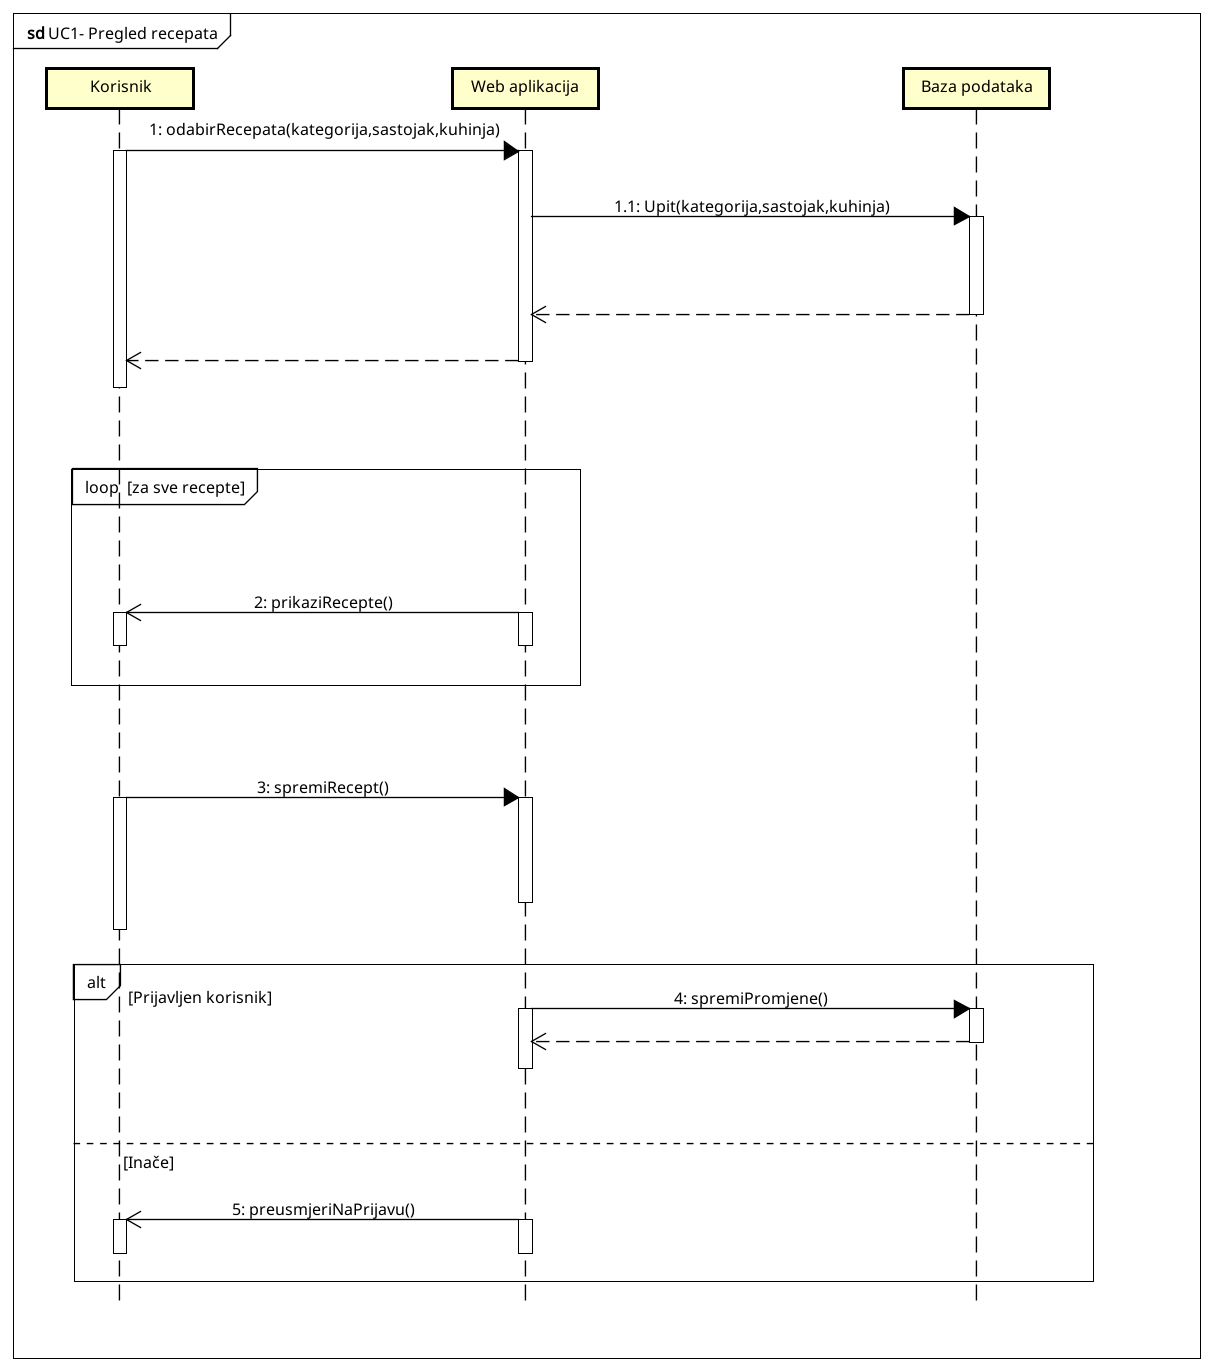
\includegraphics[scale= 0.4]{slike/sekvencijski_dijagramUC1.png}
					\centering
					\caption{Sekvencijski dijagram za UC1}
					\label{fig:Sekvencijski dijagram za UC1}
				\end{figure} 
				\eject

				\noindent
				\textbf{Obrazac uporabe UC3-Registracija}\newline
					{Korisnik se registrira s korisničkim imenom i lozinkom. Ako takav korisnik već postoji, korisniku se ispisuje greška. Inače, korisnik se uspješno registrirao i to se bilježi u bazi podataka.}
				

				\begin{figure}[H]
					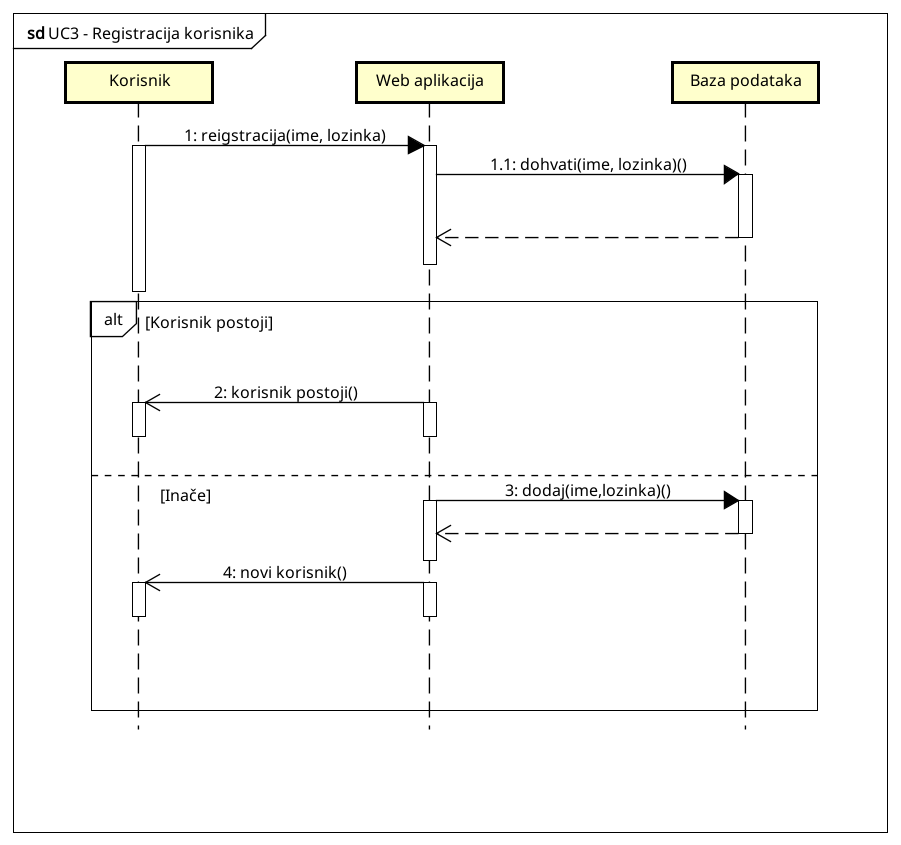
\includegraphics[scale= 0.6]{slike/sekvencijski_dijagramUC3.png}
					\centering
					\caption{Sekvencijski dijagram za UC3}
					\label{fig:Sekvencijski dijagram za UC3}
				\end{figure}
				
				\eject

				\noindent
				\textbf{Obrazac uporabe UC4-Prijava Korisnika}\newline
					{Korisnik pokuša objaviti novi recept. Ako nije prijavljen, preusmjeri ga se na prijavu. Inače, recept se dodaje u bazu podataka i o tome se obavijesti korisnik.}
				

				\begin{figure}[H]
					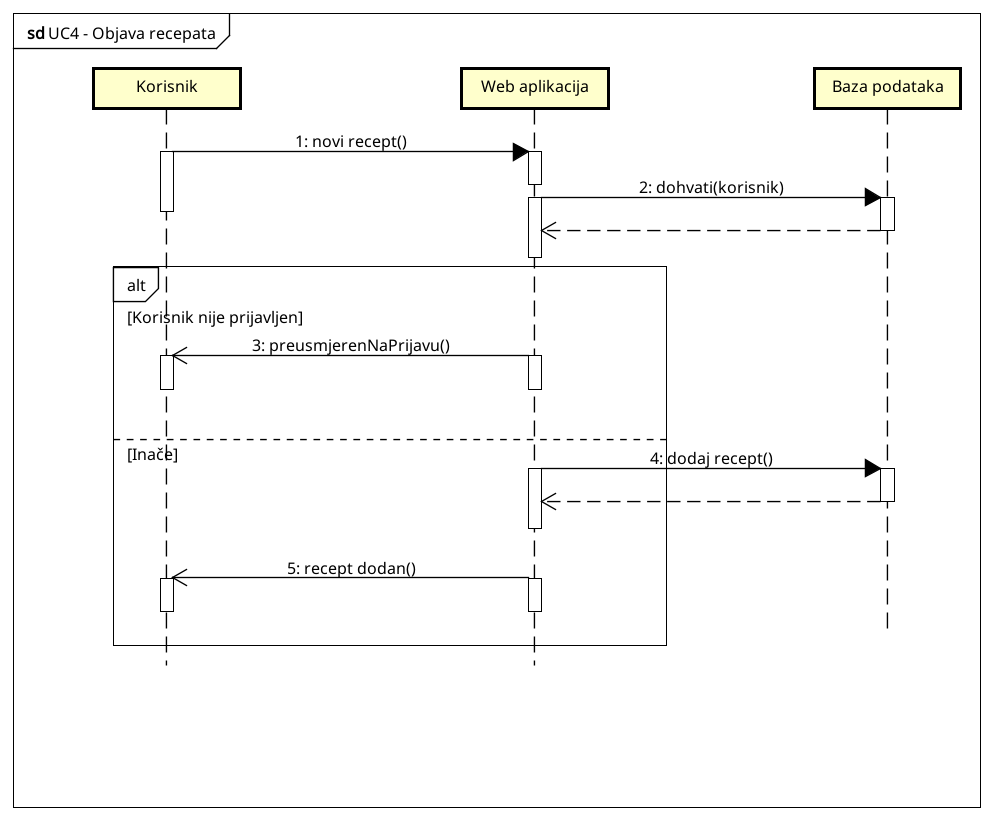
\includegraphics[scale= 0.6]{slike/sekvencijski_dijagramUC4.png}
					\centering
					\caption{Sekvencijski dijagram za UC4}
					\label{fig:Sekvencijski dijagram za UC4}
				\end{figure}

				\eject

				\noindent
				\textbf{Obrazac uporabe UC8-Videopoziv}\newline
					{Korisnik zatraži video poziv s drugim korisnikom. Ako drugi korisnik ne postoji, poziv se ne uspostavlja i o tome se obavijesti prvog korisnika. Inače se šalje zahtjev za video pozivom drugom korisniku, koji ga može odbiti ili prihvatiti. Ako odbije poziv se ne uspostavlja i o tome se obavijesti prvi korsnik. Ako prihvati uspostavi se video poziv između dva korisnika.}
				

				\begin{figure}[H]
					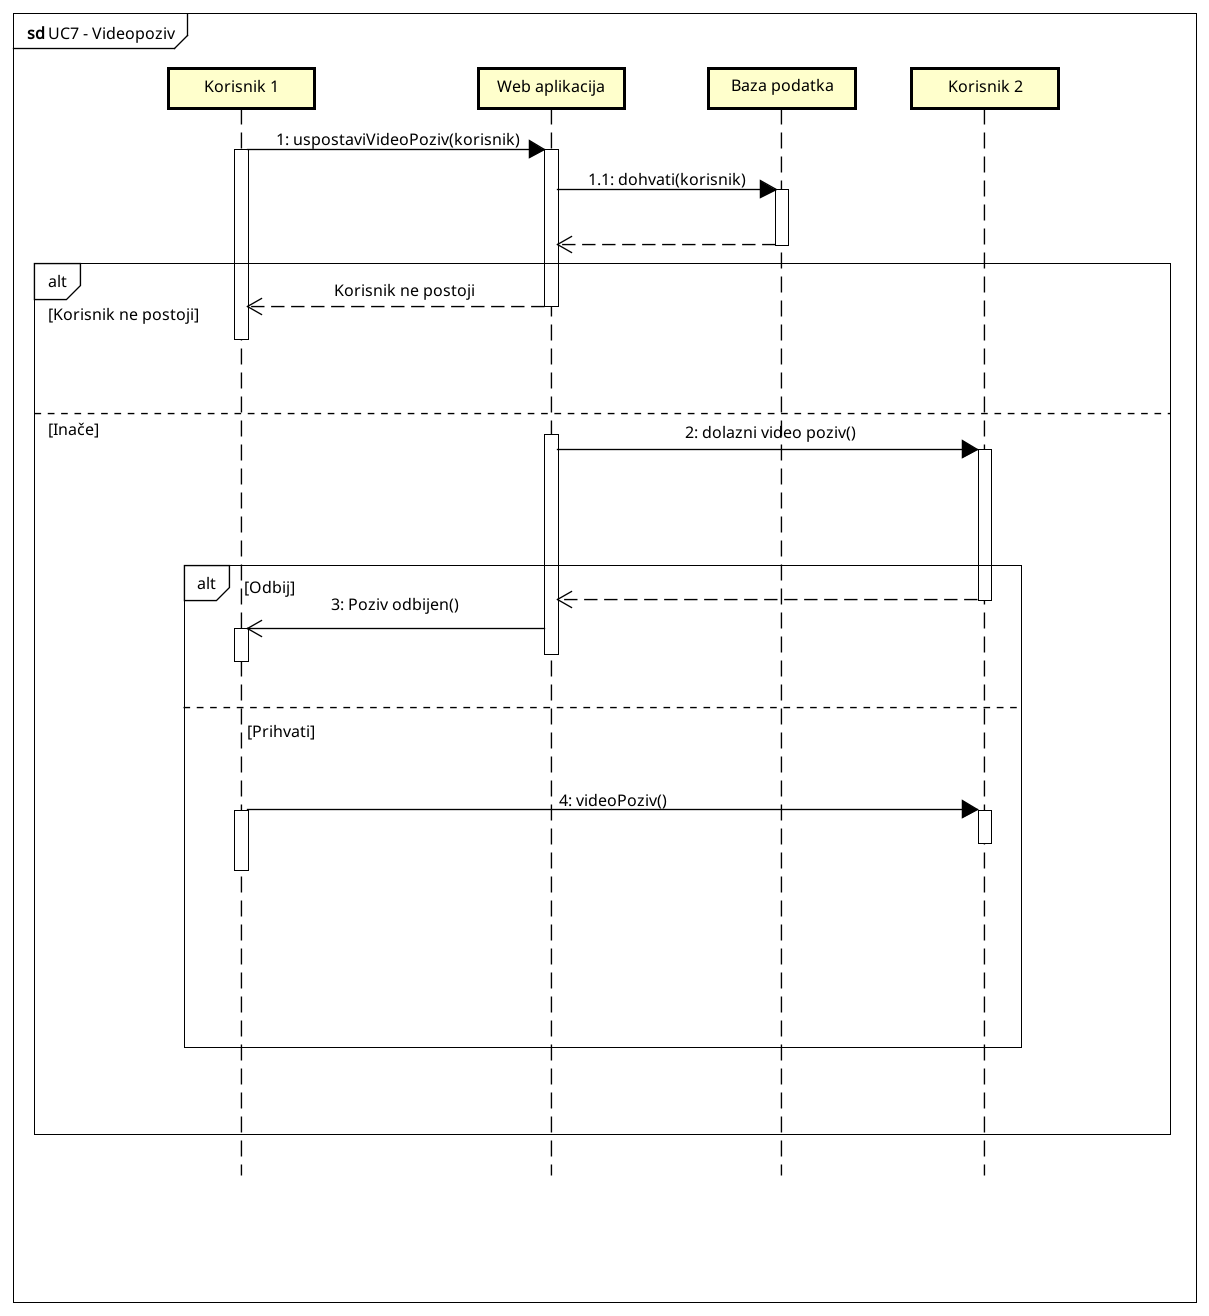
\includegraphics[scale= 0.5]{slike/sekvencijski_dijagramUC7.png}
					\centering
					\caption{Sekvencijski dijagram za UC7}
					\label{fig:Sekvencijski dijagram za UC7}
				\end{figure}
				
				\eject
			
			\section{Ostali zahtjevi}
		
			\textit{Nefunkcionalne zahtjeve koji će se navesti u nastavku teksta pojašnjavaju dodatne zahtjeve koje web aplikacija treba koristiti ili već koristi.}
			
			\begin{packed_item}
				
				\item Sustav treba biti implementiran kao web aplikacija koristeći objektno-orijentirane paradigme i norme kako bi se omogućilo ponovno korištenje dijelova koda/modula.
				\item Nepravilno korištenje web aplikacije ne smije rezultirati padom sustava, odnosno potrebno je usmjeriti korisnika na pravilno korištenje informacionim obavještenjima.
				\item U sustavu treba biti omogućen rad i korištenje web aplikacije od strane više korisnika (cca. 50).
				\item Sustav treba omogućiti komuniciranje korisnika s ostalim korisnicima putem tekstualnog chat-a i video poziva.
				\item Sustav mora podržati dijakritičke znakove hrvatskoj jezika, dakle treba podržati hrvatsku abecedu. Omogućit će se i promjena jezika s hrvatskog na engleski jezik.
				\item Hrvatski jezik je zadani jezik unutar web aplikacije.
				\item Sustav mora imati intuitivno sučelje koje neće stvarati nedoumice kod korisnika odnosno web-aplikacija treba biti jednostavna za korištenje.
				\item Konekcija s bazom podataka mora imati brz odziv. Bilo kakav pokušaj neovlaštenog pristupa informacijama u bazi podataka potrebno je spriječiti i istu adekvatno zašititi.
				\item Web aplikacija koristi proces kripitiranja lozinki za prijavu korisnika koji se tako u hash-ovima spremaju u bazu podataka.
				\item Sustav mora omogućiti korištenje određenih funkcionalnosti samo prijavljenim/registriranim korisnicima.
				\item Učitavanje početne stranice web aplikacije ne smije trajati duže od 5 sekundi.
				\item Pristup sustavu i razmjena podataka se vrši HTTPS protokolom.
				\item Pri razvoju web aplikacije koristi se React Native i Spring framework u Java programskom jeziku.
				
			\end{packed_item}
			 
			 
			 
	